\documentclass[11pt]{article}
%\documentclass[12pt]{proc}
\usepackage{graphicx}    % includes epsf
\usepackage{hyperref}
\usepackage{booktabs}
\usepackage{multirow}
\usepackage{siunitx}
\usepackage{threeparttable}
\usepackage{tabularx}

\newcommand{\ra}[1]{\renewcommand{\arraystretch}{#1}}

\addtolength{\oddsidemargin}{-0.75in}
\addtolength{\evensidemargin}{-0.5in}
\addtolength{\textwidth}{1.25in}
\addtolength{\topmargin}{-0.5in}
\addtolength{\textheight}{1in}

\begin{document}
%\onecolumn
\title{Beam parameters for the Hall-B RG-D run period during fall of 2023}
\author{}
\date{\today}
\maketitle

Hall-B Run Group D is scheduled to run in the fall of 2023 in experimental Hall B. The CLAS12 is a multipurpose detector system based on a toroidal (forward detector) and a solenoid (central  detector) superconducting magnets. The detector system includes Cherenkov Counters, Drift Chambers, Scintillator Counters, Silicon-strip detectors, Micro-mega gas detectors, and Calorimeters. In this run period CLAS12 will be used in its standard detector and shielding configuration with the Forward tagger (FT) {\bf off} and the Large M{\o}ller cone installed. RG-D run will use up to 11 GeV (5 passes) polarized electron beam, with currents up to 200 nA during the luminosity scans. This run will use several different targets ranging from cryogenic liquid targets, to heavy solid targets. Targets will be located inside the vacuum scattering chamber that is installed inside the central detector in the center of the 5 T solenoid magnet. 


\begin{table*}
\caption{Target configurations that will be used in RG-D where liquid targets are denoted by "L" and solid targets are listed just as the chemical composition.}\label{tb:target}
\centering
%\footnotesize
\begin{tabular}{@{}p{1cm}p{1.8cm}p{1.8cm}p{2cm}p{2cm}p{1.5cm}p{1cm}p{1.5cm}@{}}
\toprule
   Energy (GeV)  & Target & Thickness (\si{\centi\metre}) &  Density (\si{\gram\per\centi\metre\cubed}) & Areal Density (\si{\milli\gram\per\centi\metre\squared}) & T/$X_o$ (\%) & Beam Current (\si{\nano\ampere}) & Luminosity\tnote{2}    ($10^{35}$ \si{\per\second \per\centi\metre\squared}) \\
    \midrule
       \addlinespace[0.3cm]
 $\leq$11 & LH$_2$     & 5      & 0.071 & 355      & 0.56  & 100 & 1.3\\ 
 & LD$_2$    & 5      & 0.164 & 820      & 0.7 & 50  & 1.5\\
 &  $^{12}$C       & 2$\times$0.2  & 2.20 & 440 & 2$\times$1.03 & 50 & 1.7 \\
 &  $^{63}$Cu/$^{118}$Sn     & 0.009/0.018   & 8.96/7.31 & 80.64/131.6 & 0.63/1.49 & 150 & 1.2\\
 & Empty  &  --   &  -- & --  & -- & 165 &  -- \\
\bottomrule
    \end{tabular}

 \end{table*}

The target system used for RG-D is the new cryo-target.  RG-D will use liquid H$_2$ and D$_2$), and also solid targets ($^{118}$Sn, $^{63}$Cu, $^{12}$C) mounted on the flag system. The targets are housed in a vacuum vessel along with the cryogenic system.  A scattering chamber is installed around the target cell area.  This is made from Rohacell foam with a wall thickness of 6.5 mm.  Aluminum windows are used at the entrance and exit of the liquid cells, and at the exit of the scattering chamber. The schematic view of the RG-D target assembly is shown in Fig.~\ref{fig:RGDT}. 

\begin{figure}[htb!]
\centering
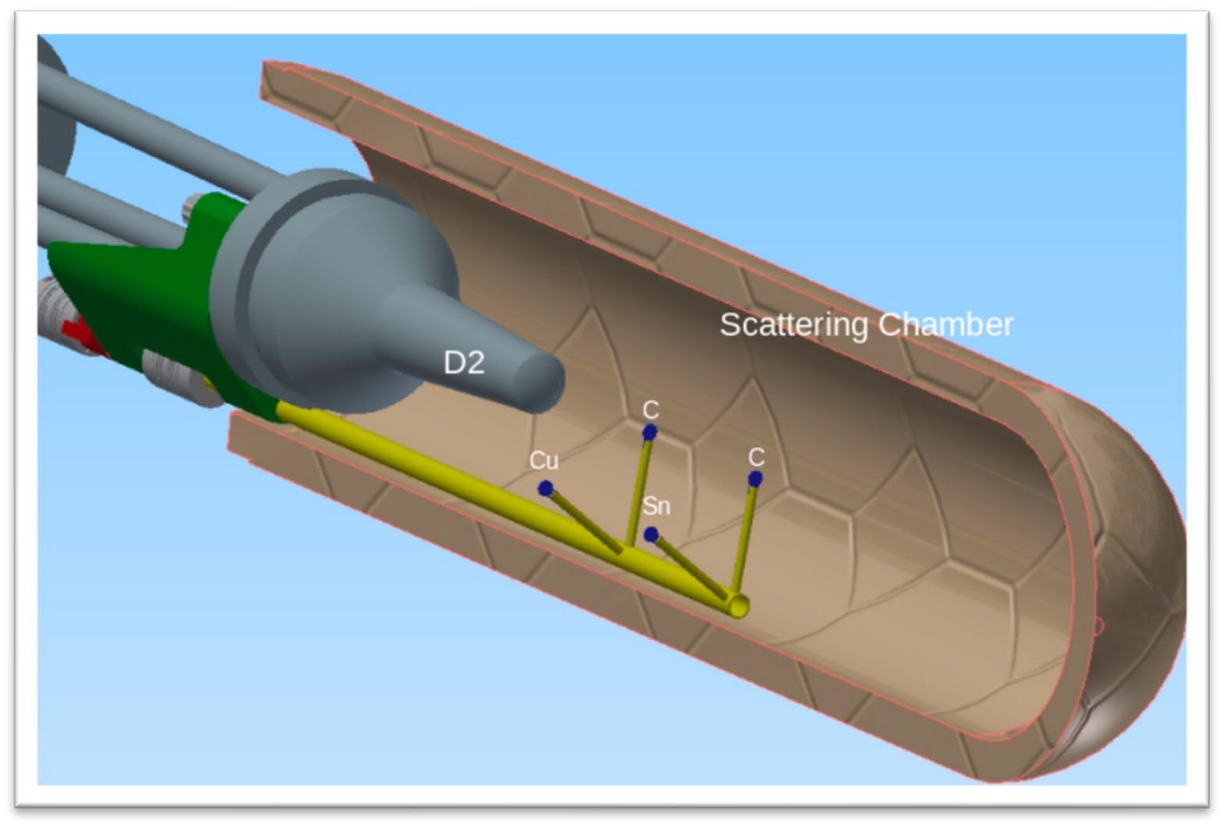
\includegraphics[width=0.8\textwidth]{RGDtarget.png}
\caption{Schematic view of the target assembly.
The flag design sowing foils 5 cm apart mounted on the same shaft with 60 degree opening between their holding needles that rotate via stepper motor.}
\label{fig:RGDT}
\end{figure}


The details of all components, such as windows and cells, are shown on the beam line drawing, including thicknesses and locations.  The beam line layout is shown in Figures~\ref{fig:beamline1}~-~\ref{fig:beamline5}.



For initial beam tuning and after extended down time ($>$8 hours) the electron beam will be  in the tagger yoke dump. After that the beam will be sent to the Faraday Cup and centered on the target.  The electron beam polarization will be measured periodically using M{\o}ller polarimeter. During Mo{\o}ller runs the beam will be in the tagger yoke dump. For beam currents for which beam power exceeds 1 kW on the Faraday Cup (90 nA at 11 GeV) the beam blocker will be inserted upstream of the Faraday Cup.

%\newpage

During RG-D run the fast machine shutdown (FSD) system will be as follows:
\begin{enumerate}
\item Solenoid magnet current, with the exception of zero field alignment runs
\item Upstream, midstream and downstream halo counters and BOM
\end{enumerate}

FSD masking must not be changed without the Hall permission.\\
The HPS halo counters and raster are not used in this run and should be always masked.\\

The requirements for beam parameters for RG-D run are summarized in Table~\ref{tab:beam_par}

 \begin{table}[htb]
\caption{Required beam parameters.}\label{tab:beam_par}
\centering
 \begin{tabular}{|c|c|l|}
\hline
Parameter & Requirement &Comments \\ \hline 
Energy (GeV) & $\leq$11   & 5 pass  \\  \hline
$\delta$p/p & $\sim 2\times 10^{-4}$ & \\ \hline 
Current (nA) & $\le 200$ & \\  \hline
$\sigma_{xy}$ ($\mu$m) &$ < 200$& As measured by 2H01 harp \\ \hline 
Position stability ($\mu$m) & $< 100$ & On 2H01 and 2H00 ($>30$nA) \\ 
&&BPMs with feedback \\ \hline
Divergence ($\mu$rad) & $< 100$&  \\ \hline 
Beam Halo ($> \pm 5\sigma$) &$< 10^{-5}$&As measured by 2H01 harp \\ \hline
Long term current stability & $< 5$ \% & For $>30$ nA, integrated \\
&&over minutes \\ \hline 
Short term bean intensity & $<10$\%& of the total power, measured \\stability (60 Hz harmonics) && with SLM and halo rates \\ \hline
Bunch charge fluctuations &$< 10$ \% & Measured with DAQ \\ \hline
Beam polarization & $\geq 85\%$&Measured with M{\o}ller polarimeter\\ \hline
 \end{tabular}
\end{table}

\begin{figure}[hbt]
\vspace{-2cm}
\begin{center}
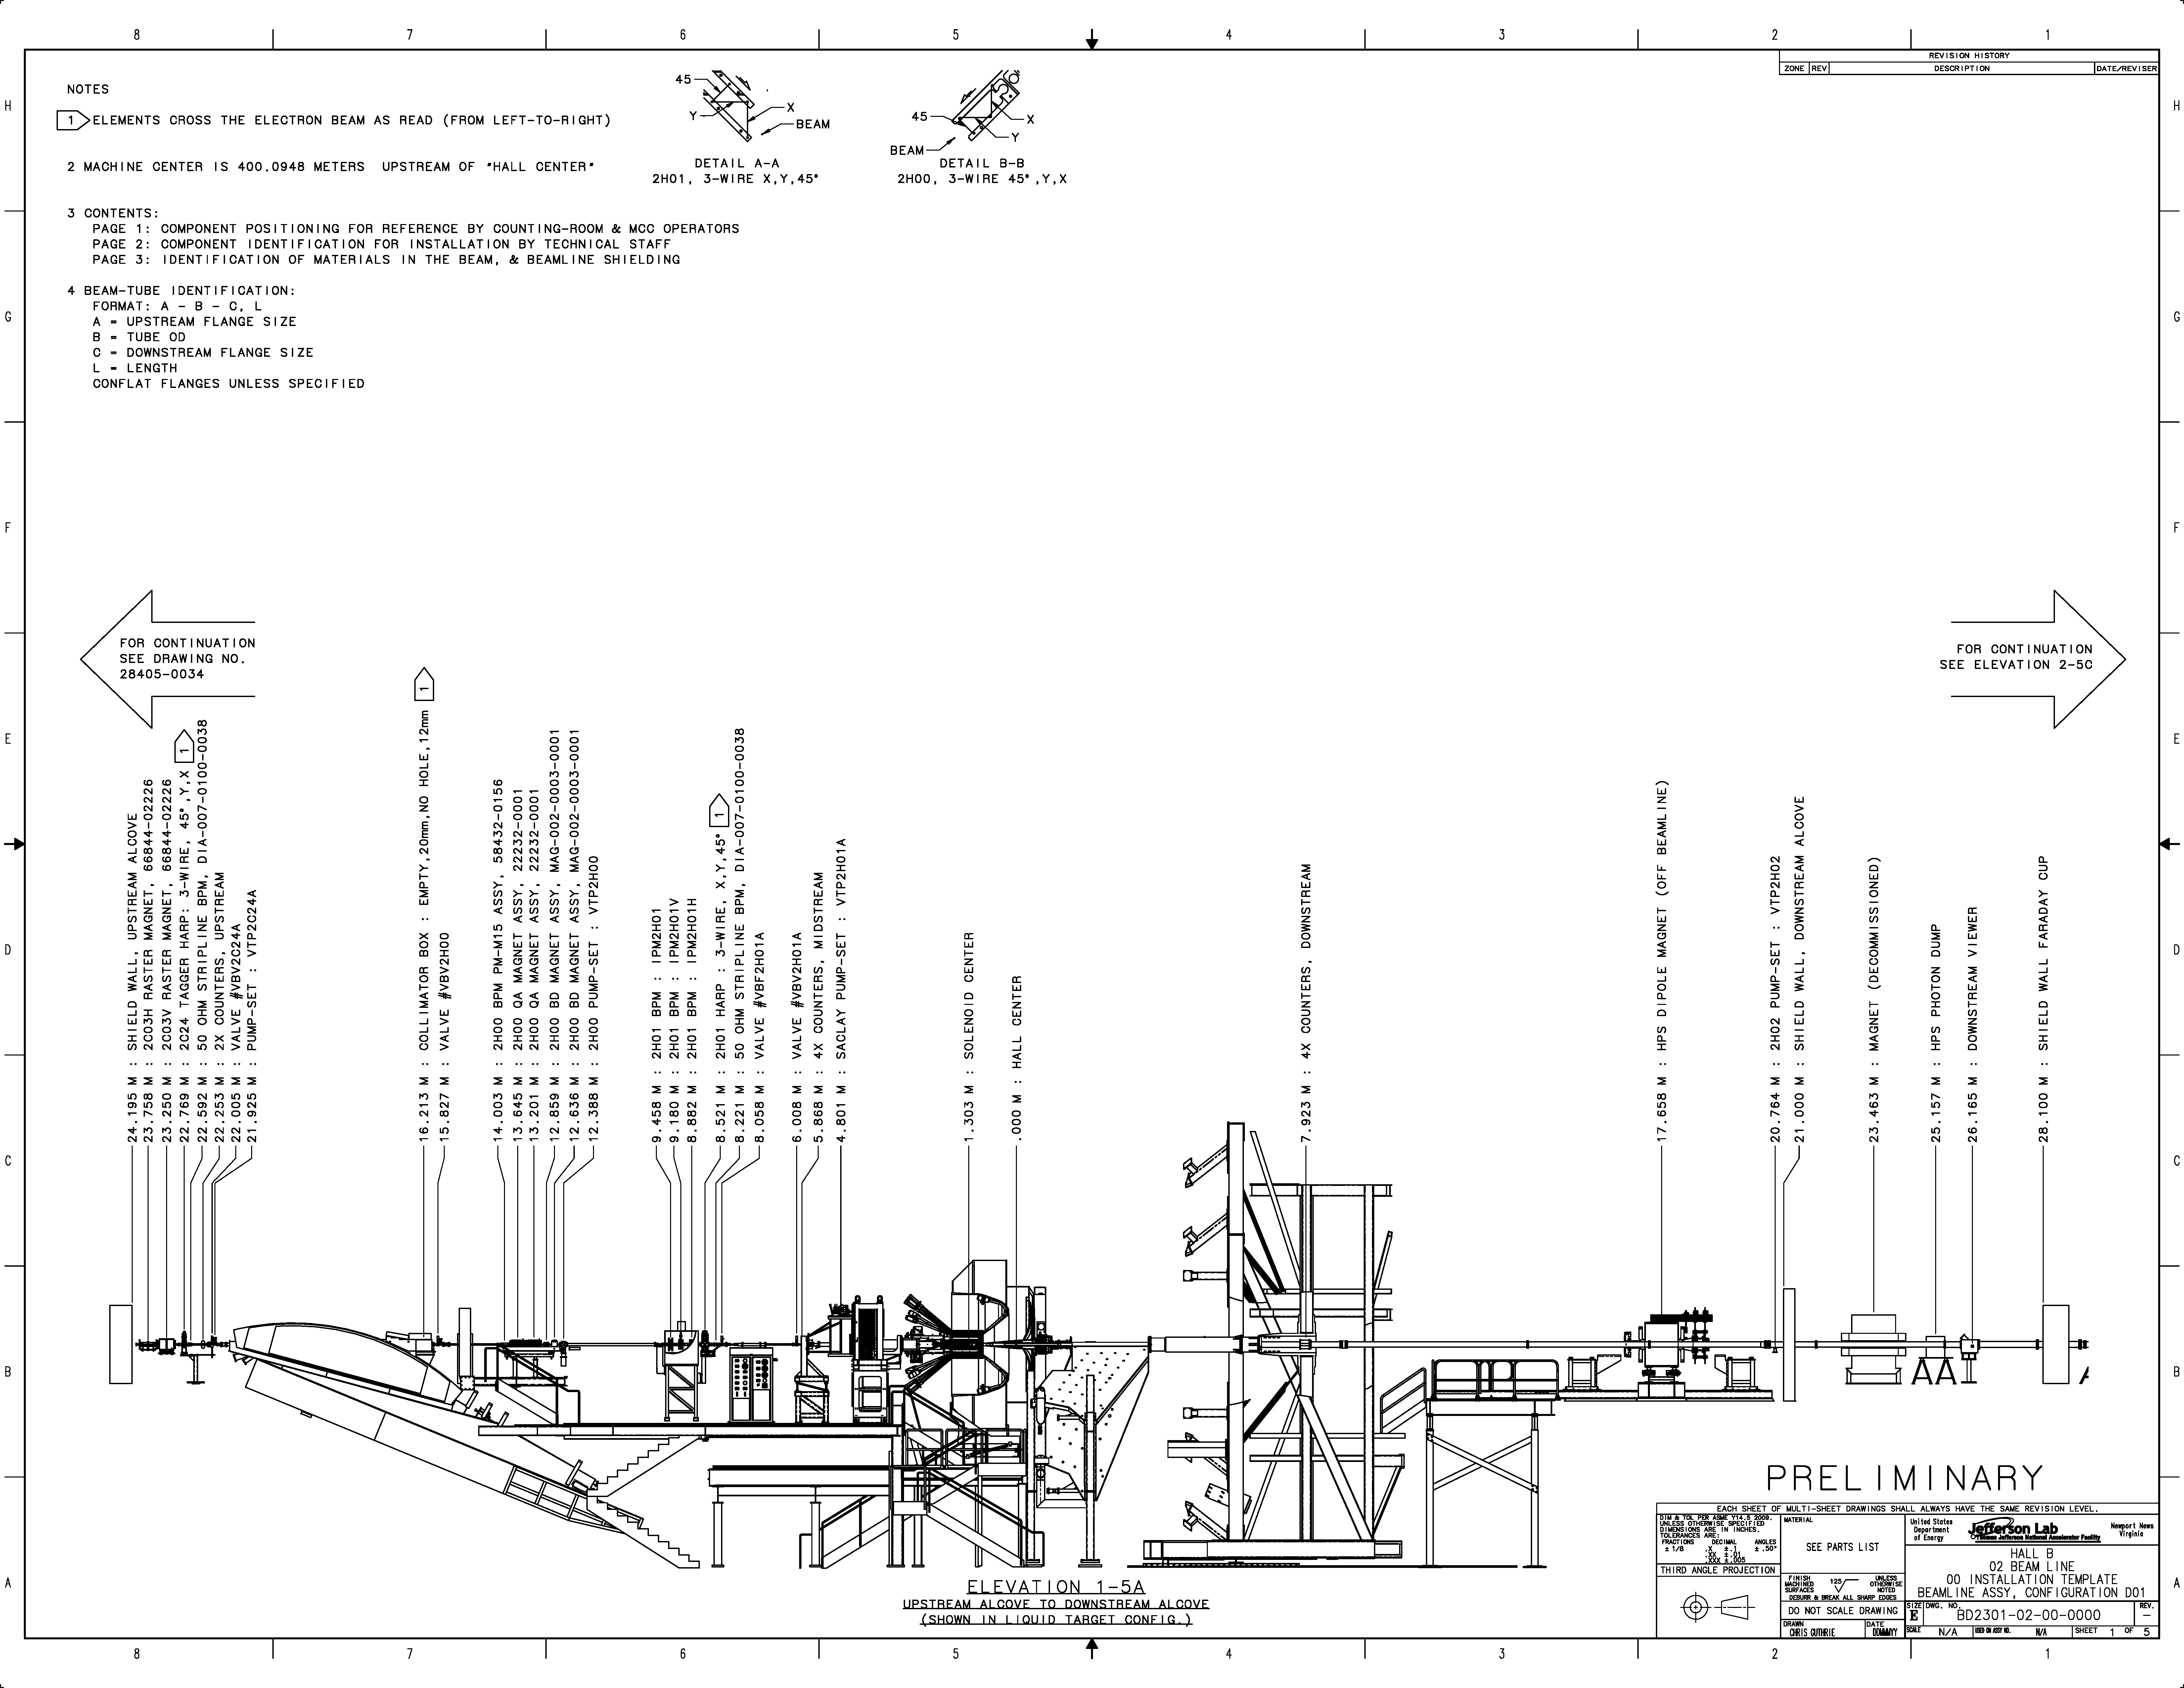
\includegraphics[width=9in,angle=90]{RGD_beamline_p1.pdf}
\caption{ \label{fig:beamline1} The layout of tHe RGD beamline. }
\end{center}
\end{figure}

\begin{figure}[hbt]
\vspace{-2cm}
\begin{center}
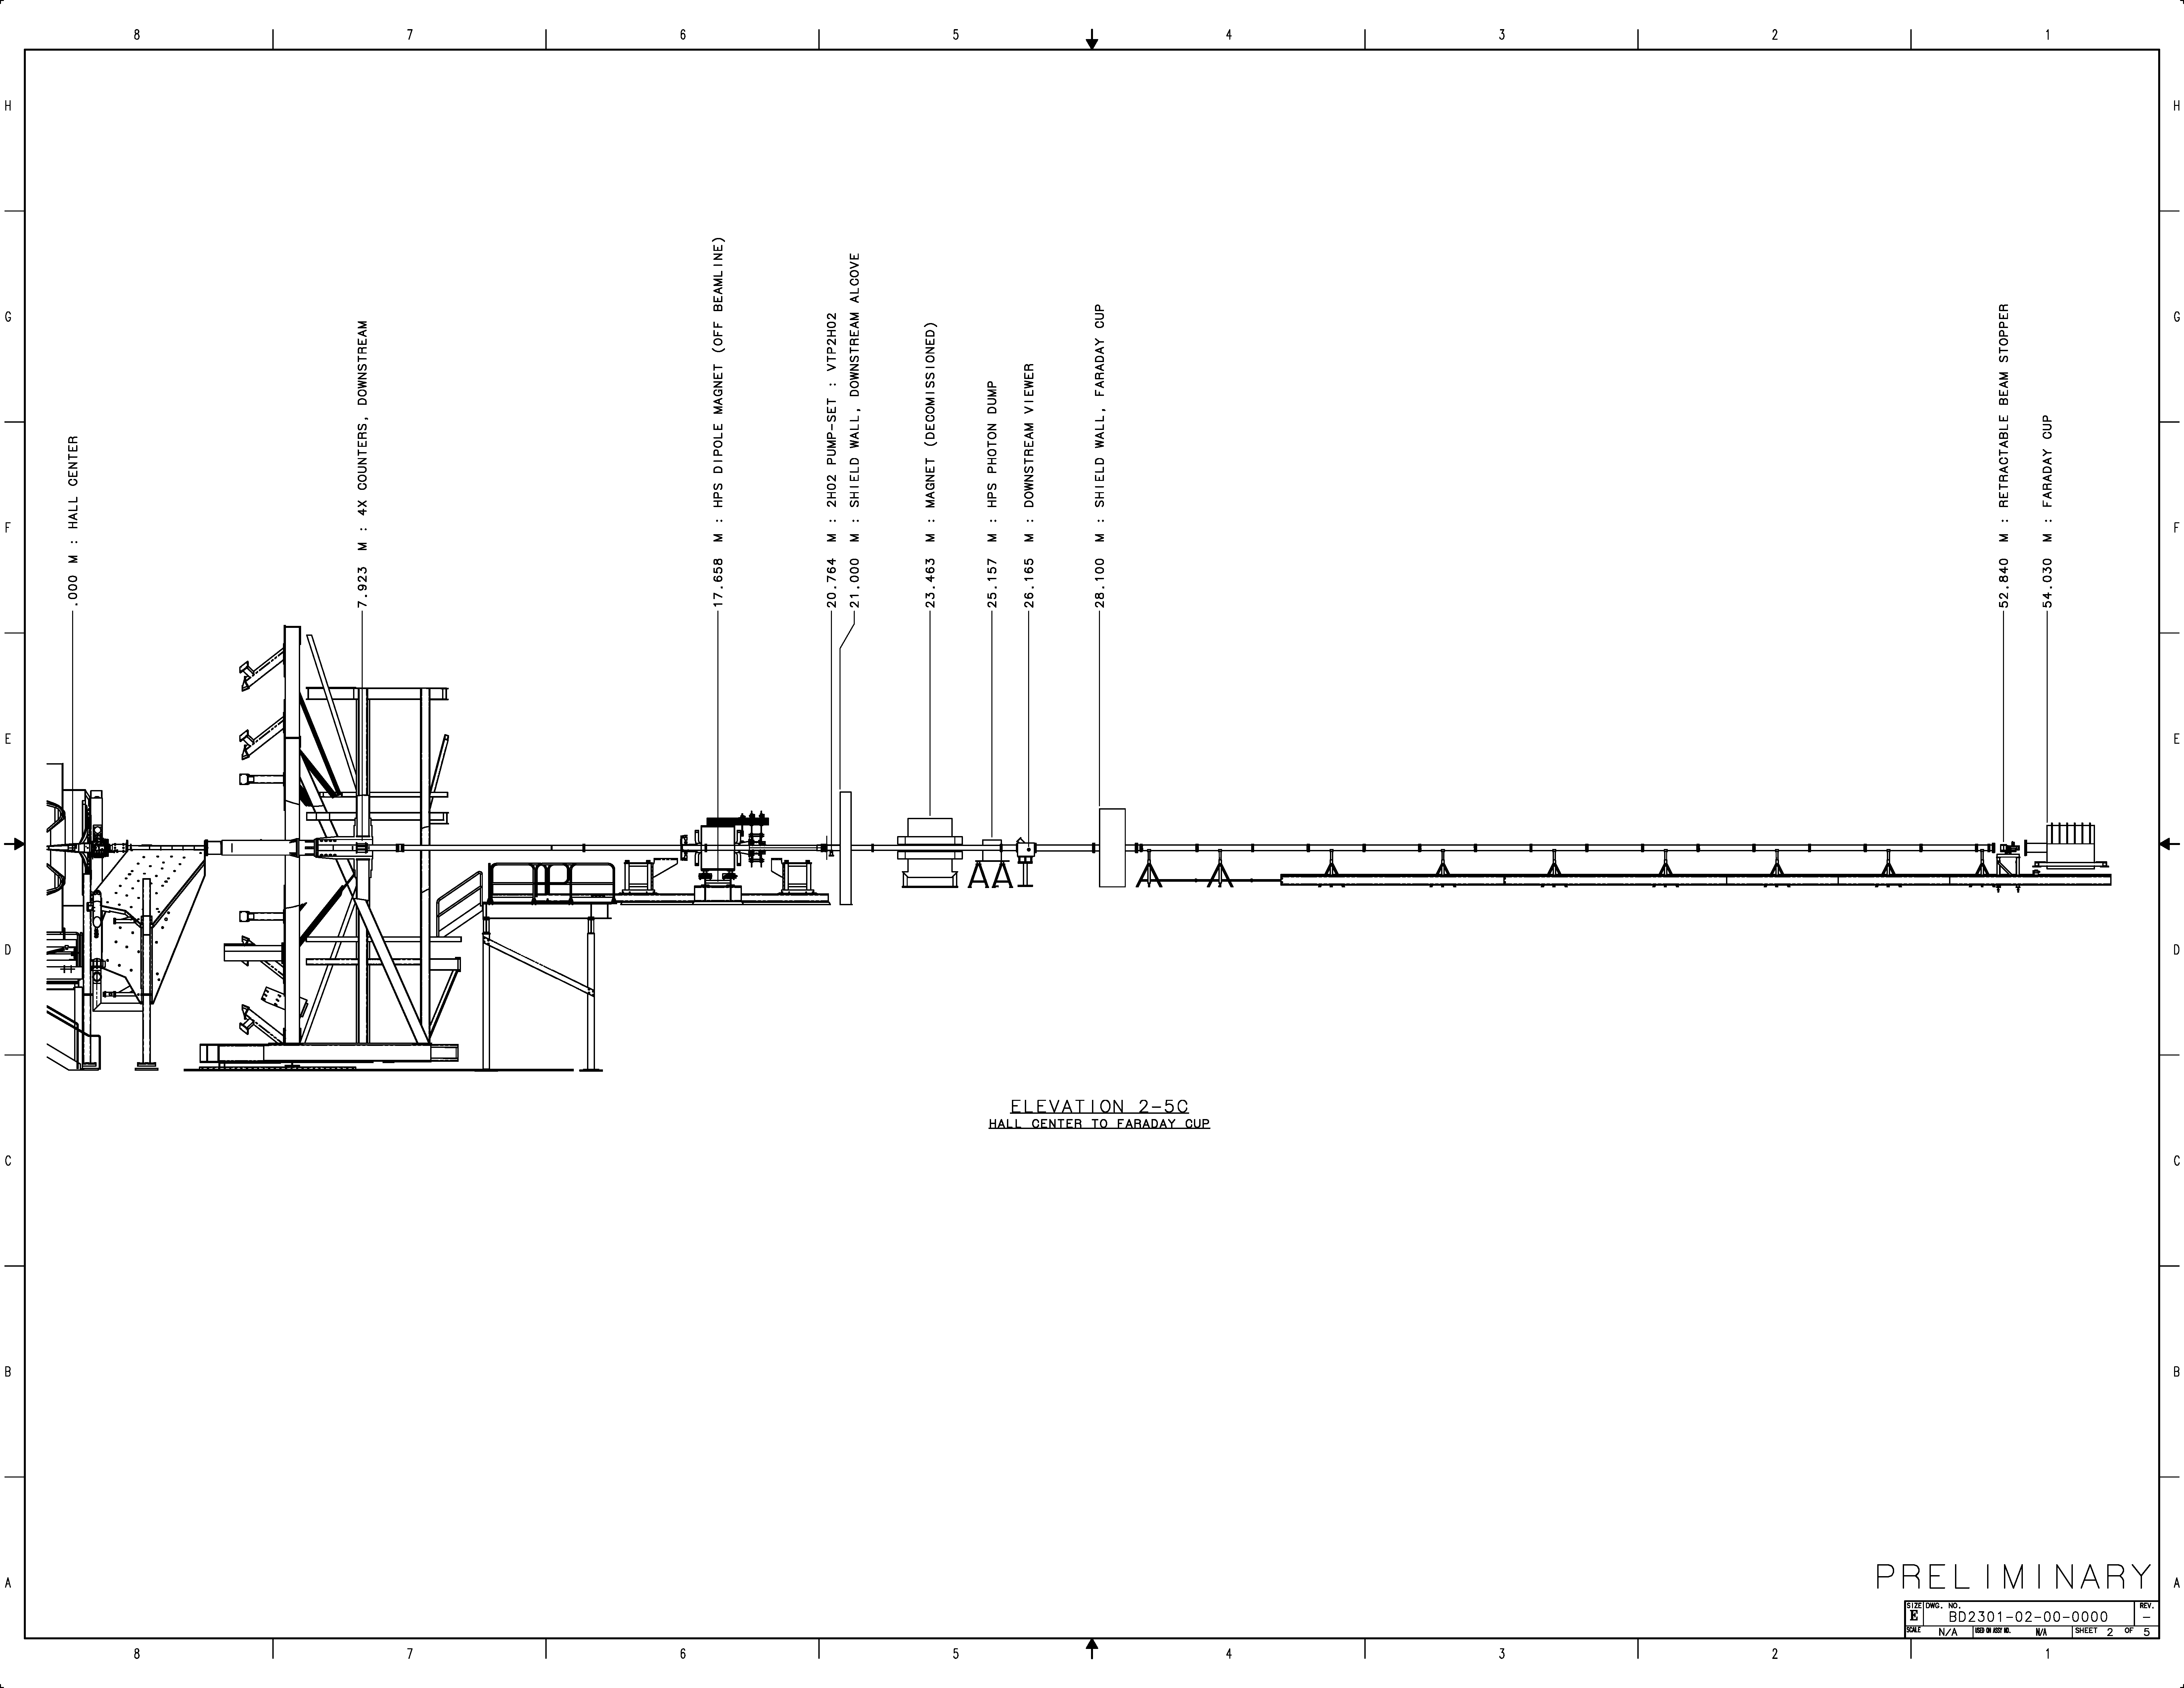
\includegraphics[width=9in,angle=90]{RGD_beamline_p2.pdf}
\end{center}
\caption{ \label{fig:beamline2} 
The layout of the RG-D beamline. }
\end{figure}

\begin{figure}[hbt]
\vspace{-2cm}
\begin{center}
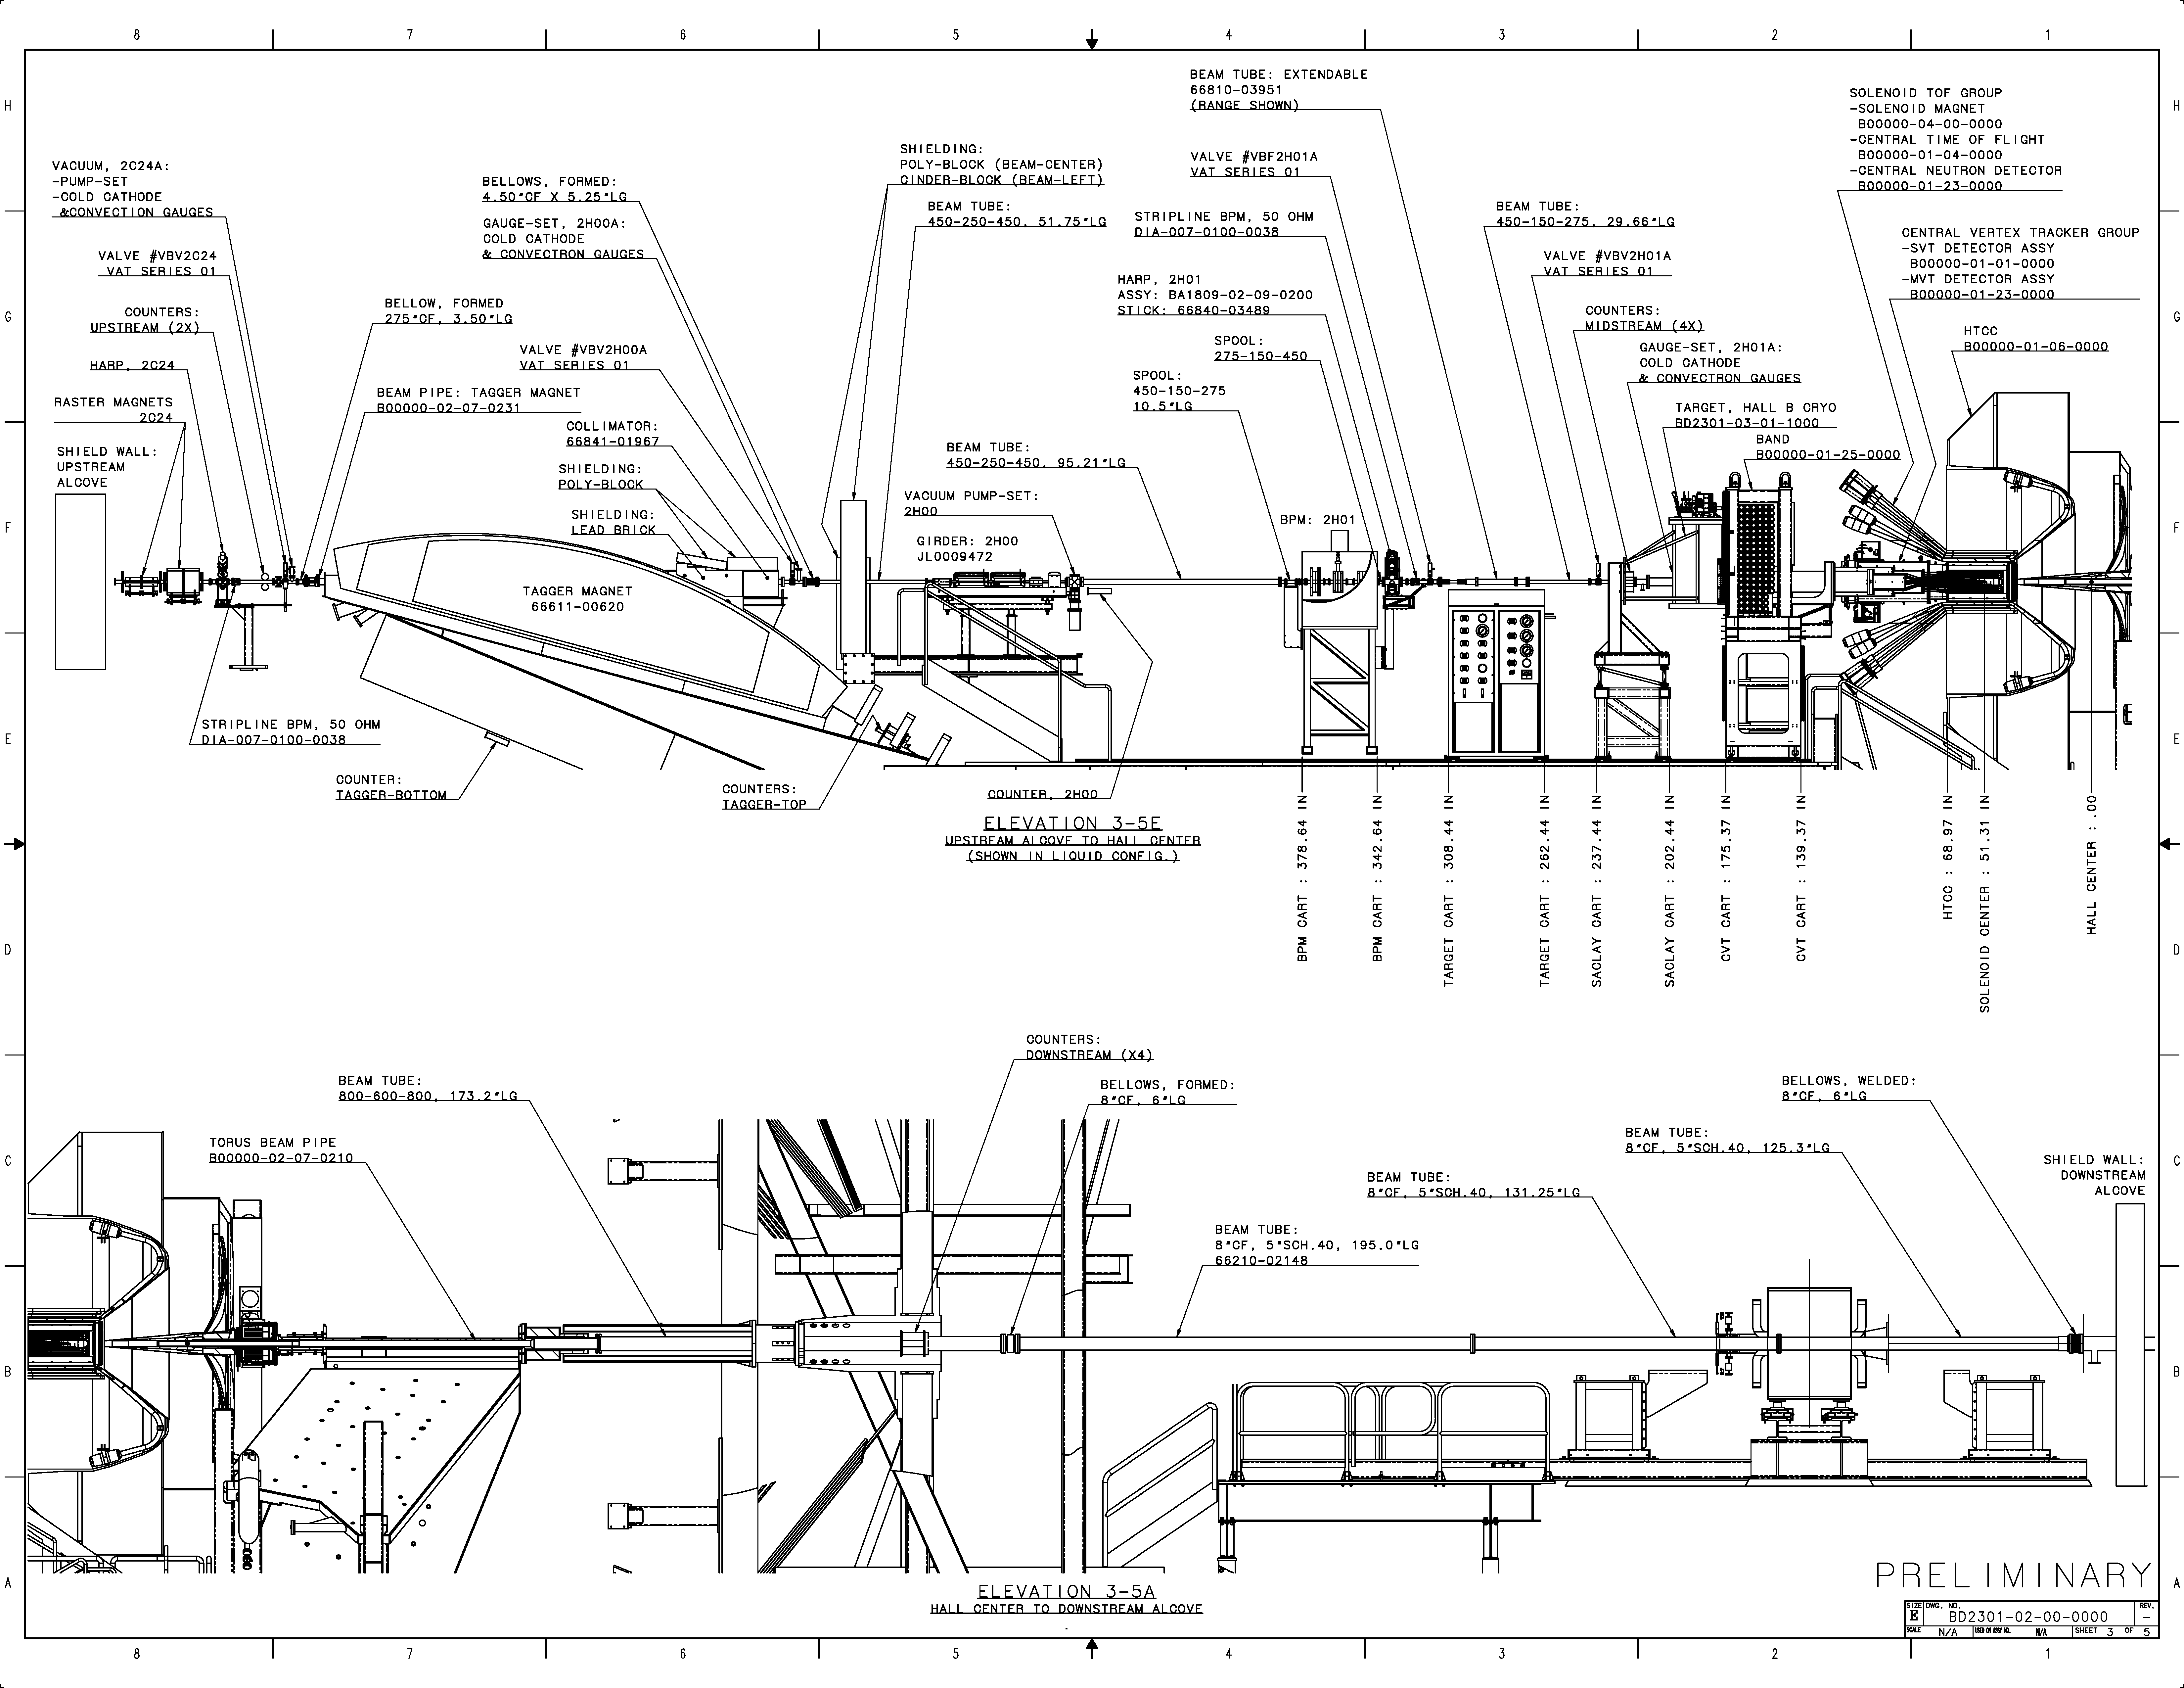
\includegraphics[width=9in,angle=90]{RGD_beamline_p3.pdf}
\end{center}
\caption{ \label{fig:beamline3} 
The layout of the RG-D beamline. }
\end{figure}

\begin{figure}[hbt]
\vspace{-2cm}
\begin{center}
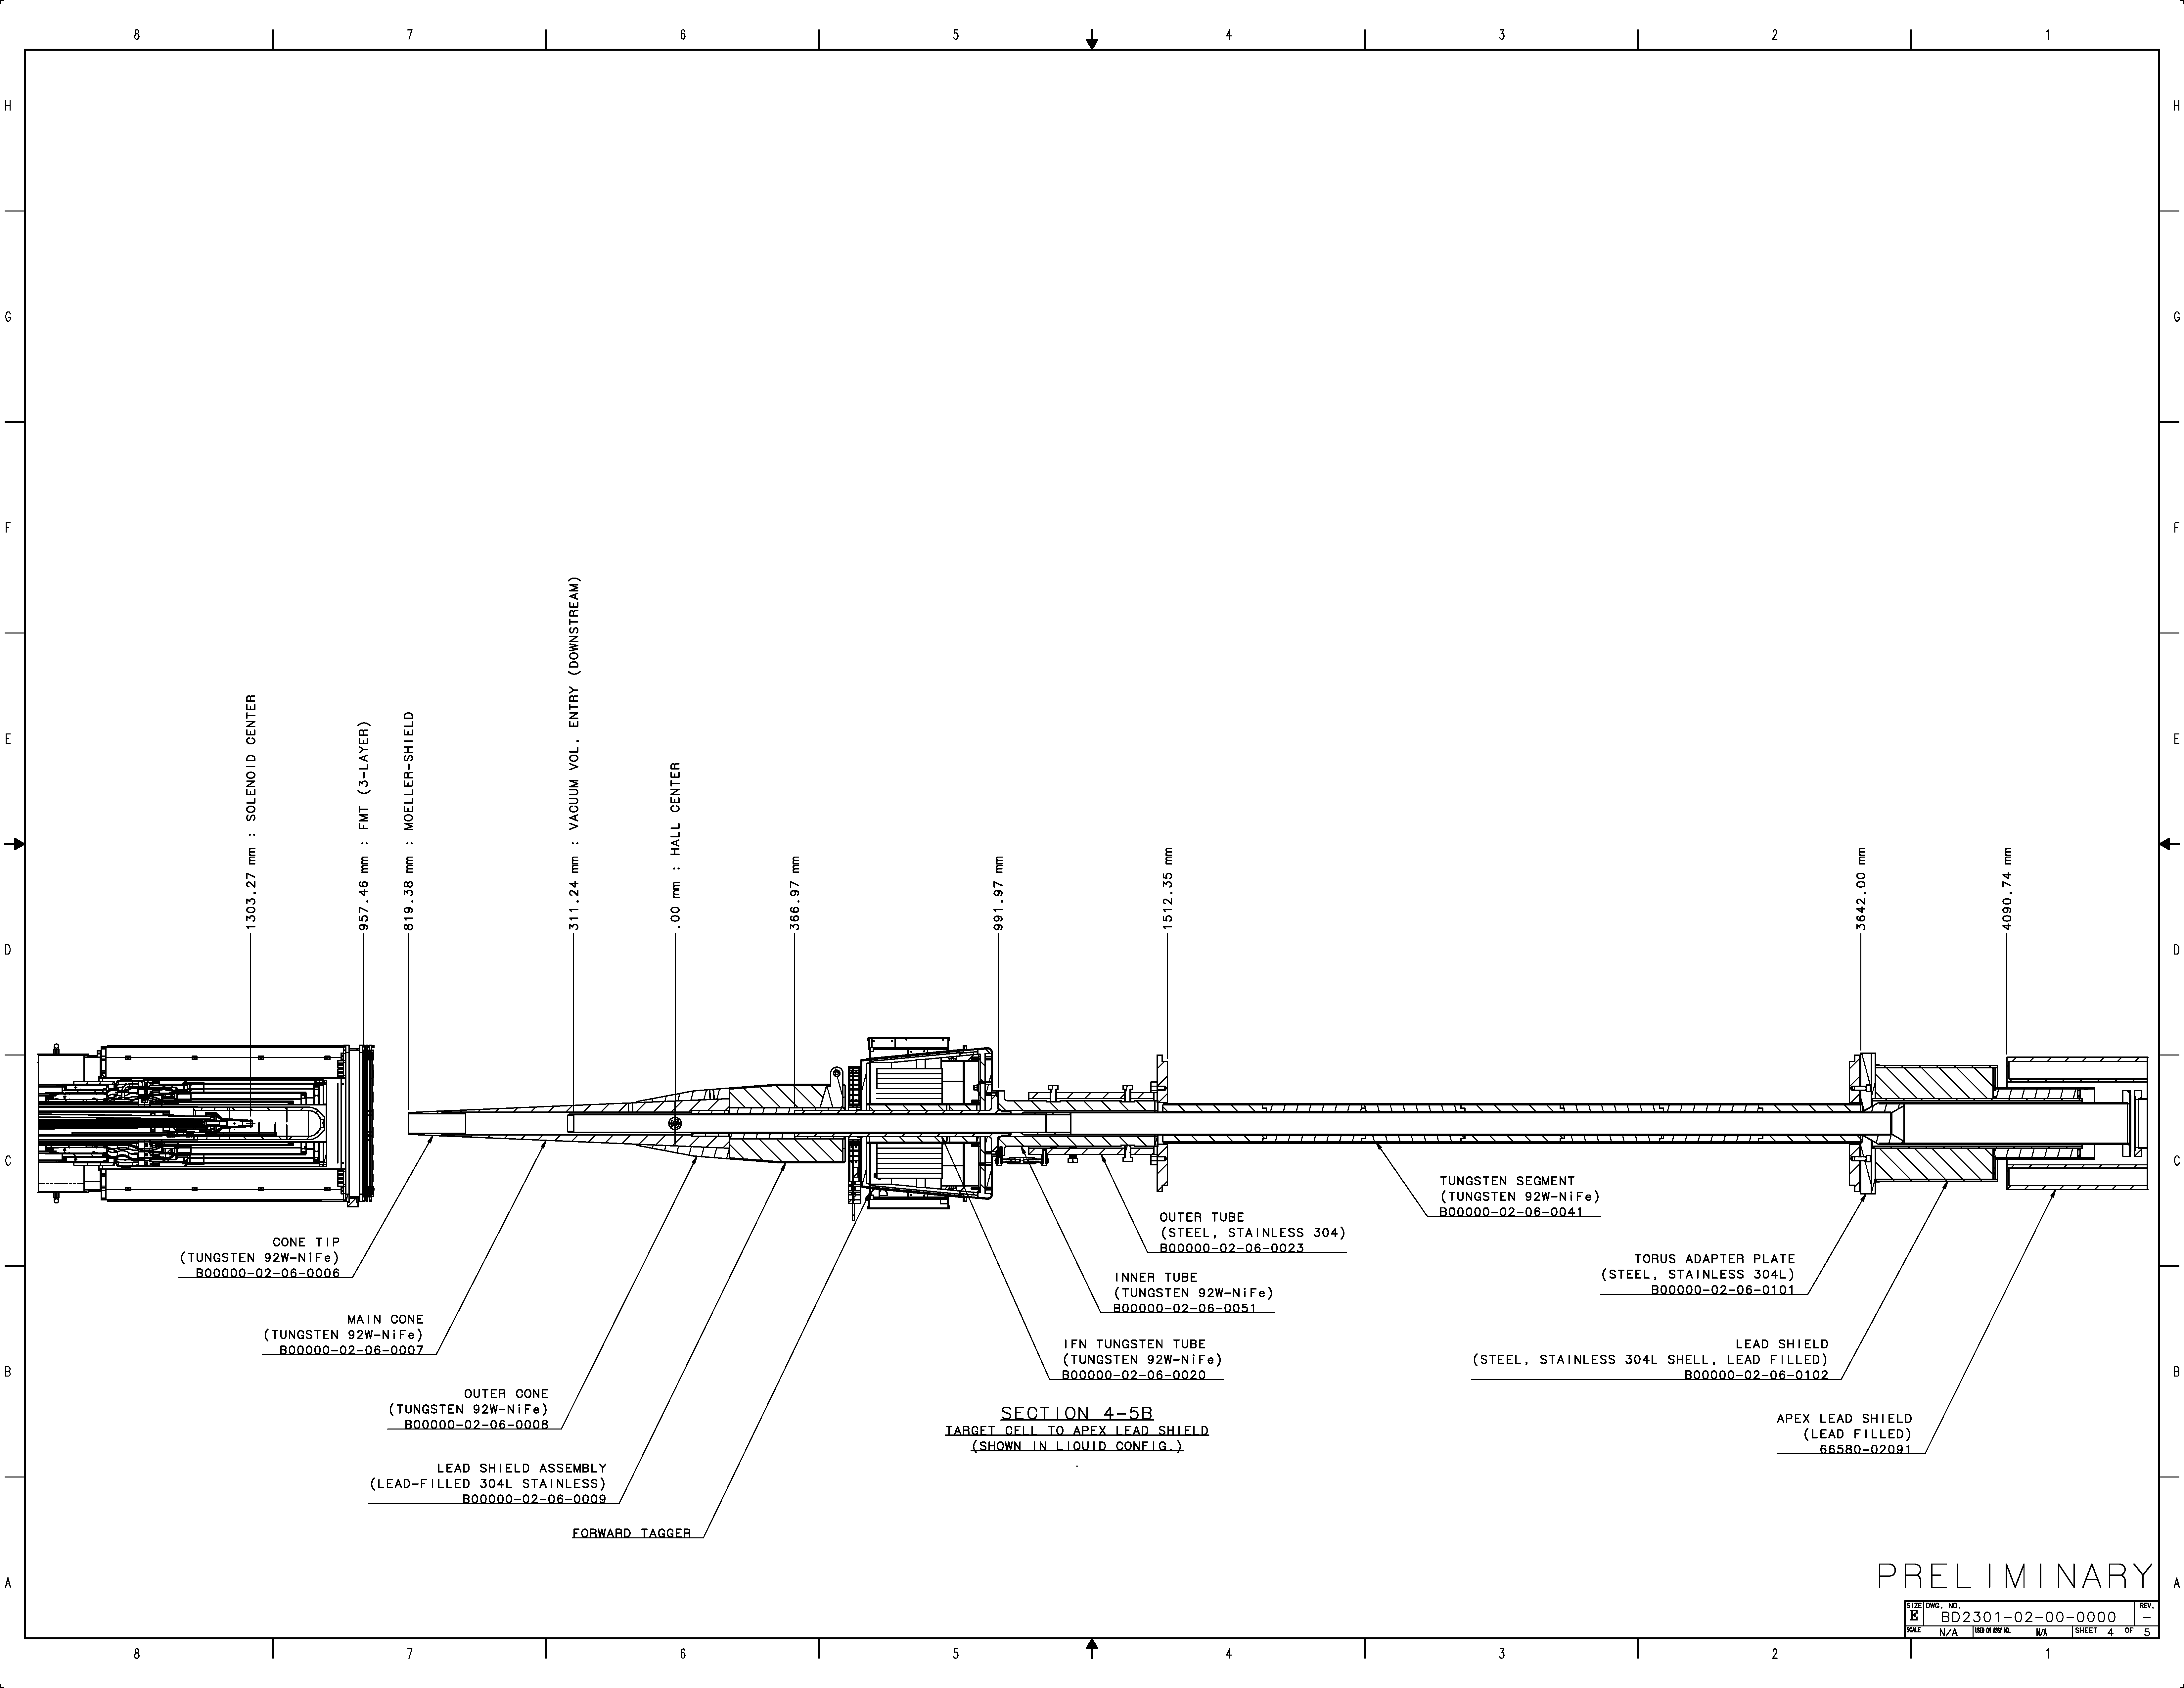
\includegraphics[width=9in,angle=90]{RGD_beamline_p4.pdf}
\end{center}
\caption{ \label{fig:beamline4}
The layout of the RG-D beamline.}
\end{figure}

\begin{figure}[hbt]
\vspace{-2cm}
\begin{center}
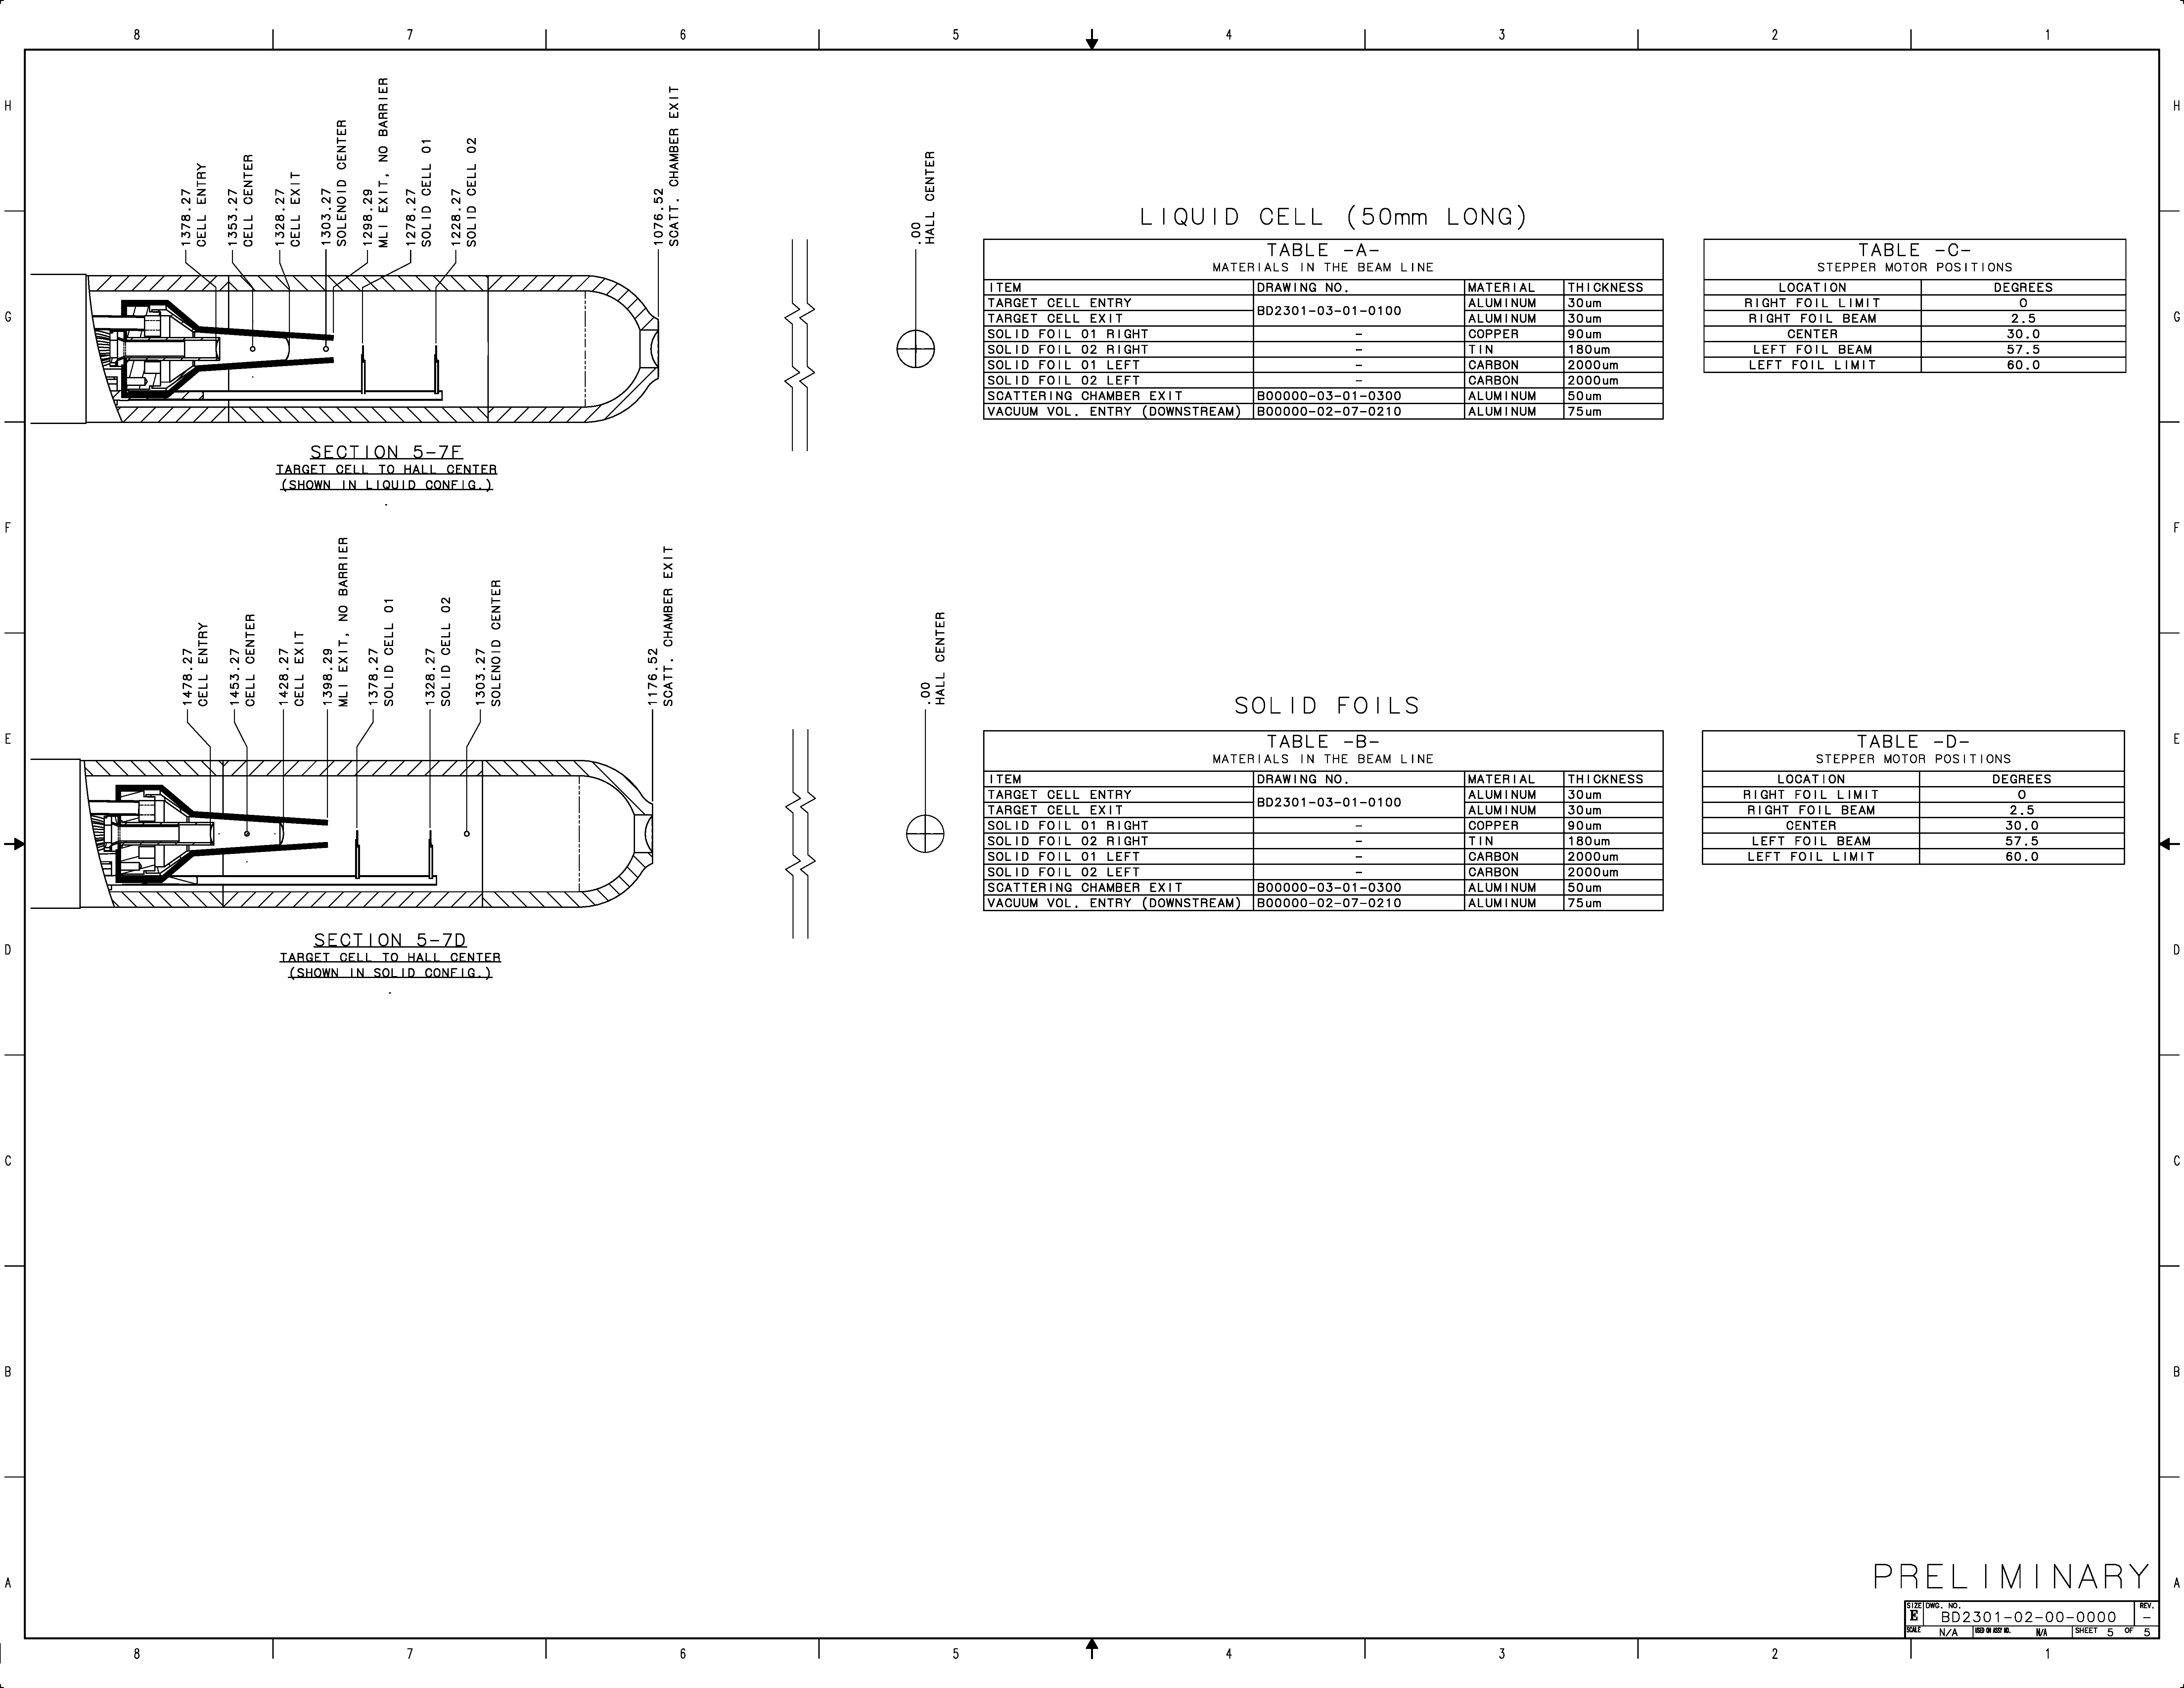
\includegraphics[width=9in,angle=90]{RGD_beamline_p5.pdf}
\end{center}
\caption{ \label{fig:beamline5} 
The layout of the RG-D beamline. }
\end{figure}


\end{document}
